% Created by tikzDevice version 0.10.1 on 2016-06-15 03:39:25
% !TEX encoding = UTF-8 Unicode
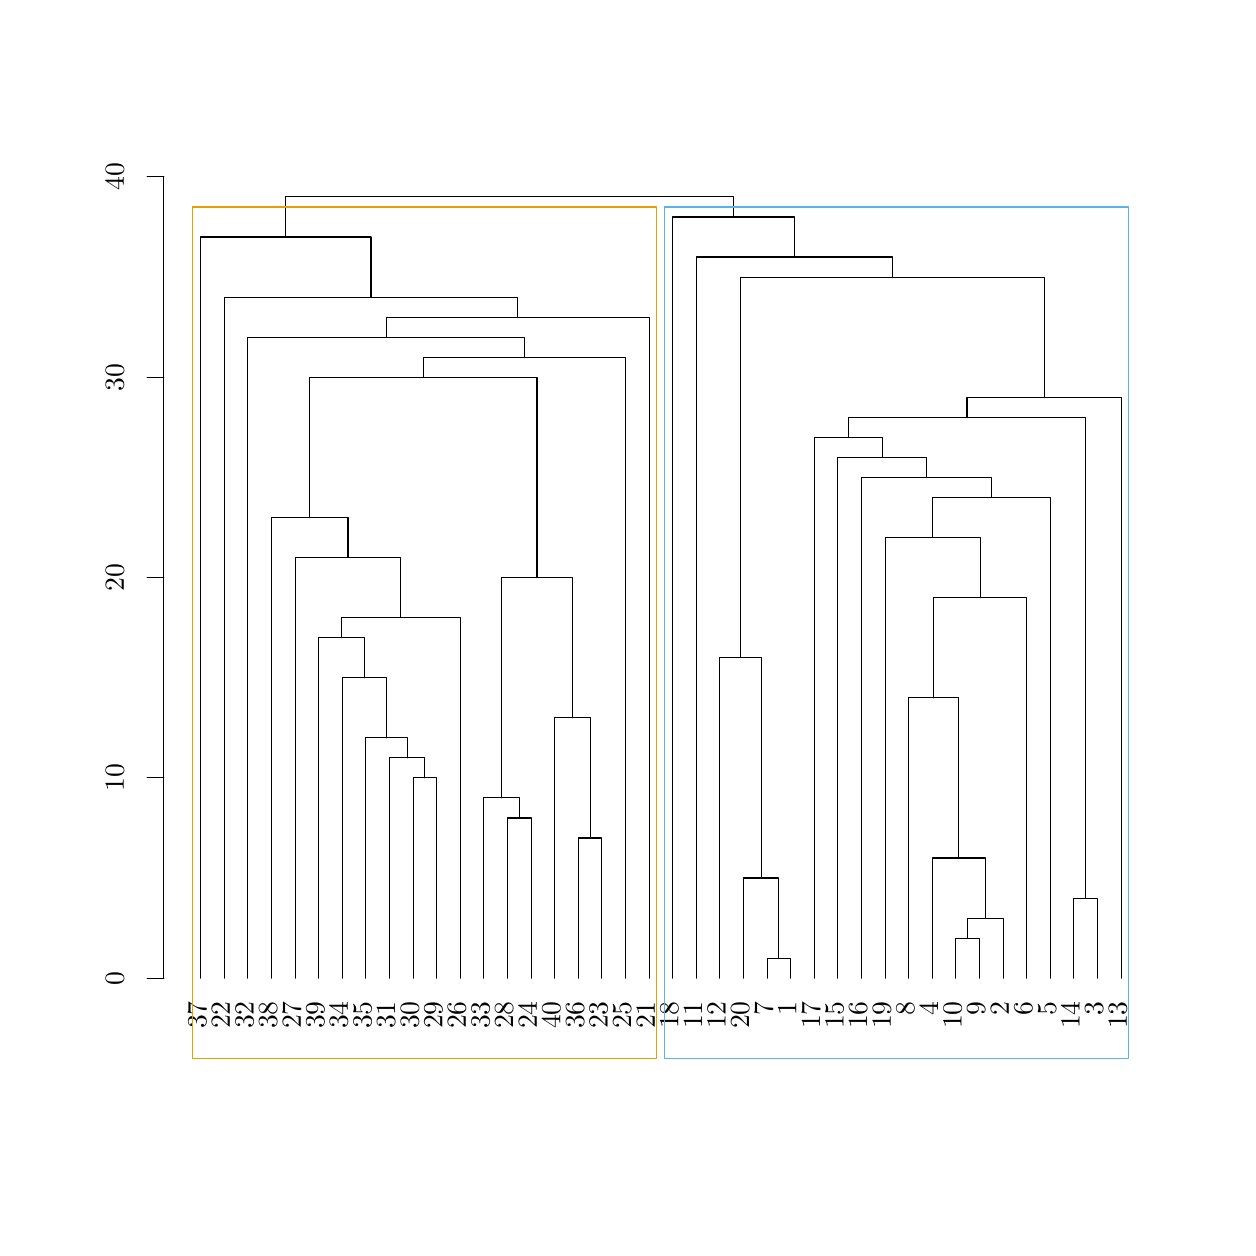
\begin{tikzpicture}[x=1pt,y=1pt]
\definecolor{fillColor}{RGB}{255,255,255}
\path[use as bounding box,fill=fillColor,fill opacity=0.00] (0,0) rectangle (433.62,433.62);
\begin{scope}
\path[clip] (  0.00,  0.00) rectangle (433.62,433.62);
\definecolor{drawColor}{RGB}{0,0,0}

\node[text=drawColor,rotate= 90.00,anchor=base east,inner sep=0pt, outer sep=0pt, scale=  1.00] at ( 64.57, 81.81) {37};

\node[text=drawColor,rotate= 90.00,anchor=base east,inner sep=0pt, outer sep=0pt, scale=  1.00] at ( 73.10, 81.81) {22};

\node[text=drawColor,rotate= 90.00,anchor=base east,inner sep=0pt, outer sep=0pt, scale=  1.00] at ( 81.63, 81.81) {32};

\node[text=drawColor,rotate= 90.00,anchor=base east,inner sep=0pt, outer sep=0pt, scale=  1.00] at ( 90.16, 81.81) {38};

\node[text=drawColor,rotate= 90.00,anchor=base east,inner sep=0pt, outer sep=0pt, scale=  1.00] at ( 98.68, 81.81) {27};

\node[text=drawColor,rotate= 90.00,anchor=base east,inner sep=0pt, outer sep=0pt, scale=  1.00] at (107.21, 81.81) {39};

\node[text=drawColor,rotate= 90.00,anchor=base east,inner sep=0pt, outer sep=0pt, scale=  1.00] at (115.74, 81.81) {34};

\node[text=drawColor,rotate= 90.00,anchor=base east,inner sep=0pt, outer sep=0pt, scale=  1.00] at (124.27, 81.81) {35};

\node[text=drawColor,rotate= 90.00,anchor=base east,inner sep=0pt, outer sep=0pt, scale=  1.00] at (132.80, 81.81) {31};

\node[text=drawColor,rotate= 90.00,anchor=base east,inner sep=0pt, outer sep=0pt, scale=  1.00] at (141.33, 81.81) {30};

\node[text=drawColor,rotate= 90.00,anchor=base east,inner sep=0pt, outer sep=0pt, scale=  1.00] at (149.86, 81.81) {29};

\path[draw=drawColor,line width= 0.4pt,line join=round,line cap=round] (139.26, 90.14) --
	(139.26,162.53) --
	(147.79,162.53) --
	(147.79, 90.14);

\path[draw=drawColor,line width= 0.4pt,line join=round,line cap=round] (130.73, 90.14) --
	(130.73,169.77) --
	(143.53,169.77) --
	(143.53,162.53);

\path[draw=drawColor,line width= 0.4pt,line join=round,line cap=round] (122.20, 90.14) --
	(122.20,177.01) --
	(137.13,177.01) --
	(137.13,169.77);

\path[draw=drawColor,line width= 0.4pt,line join=round,line cap=round] (113.68, 90.14) --
	(113.68,198.72) --
	(129.67,198.72) --
	(129.67,177.01);

\path[draw=drawColor,line width= 0.4pt,line join=round,line cap=round] (105.15, 90.14) --
	(105.15,213.20) --
	(121.67,213.20) --
	(121.67,198.72);

\node[text=drawColor,rotate= 90.00,anchor=base east,inner sep=0pt, outer sep=0pt, scale=  1.00] at (158.38, 81.81) {26};

\path[draw=drawColor,line width= 0.4pt,line join=round,line cap=round] (113.41,213.20) --
	(113.41,220.44) --
	(156.32,220.44) --
	(156.32, 90.14);

\path[draw=drawColor,line width= 0.4pt,line join=round,line cap=round] ( 96.62, 90.14) --
	( 96.62,242.15) --
	(134.86,242.15) --
	(134.86,220.44);

\path[draw=drawColor,line width= 0.4pt,line join=round,line cap=round] ( 88.09, 90.14) --
	( 88.09,256.63) --
	(115.74,256.63) --
	(115.74,242.15);

\node[text=drawColor,rotate= 90.00,anchor=base east,inner sep=0pt, outer sep=0pt, scale=  1.00] at (166.91, 81.81) {33};

\node[text=drawColor,rotate= 90.00,anchor=base east,inner sep=0pt, outer sep=0pt, scale=  1.00] at (175.44, 81.81) {28};

\node[text=drawColor,rotate= 90.00,anchor=base east,inner sep=0pt, outer sep=0pt, scale=  1.00] at (183.97, 81.81) {24};

\path[draw=drawColor,line width= 0.4pt,line join=round,line cap=round] (173.37, 90.14) --
	(173.37,148.05) --
	(181.90,148.05) --
	(181.90, 90.14);

\path[draw=drawColor,line width= 0.4pt,line join=round,line cap=round] (164.85, 90.14) --
	(164.85,155.29) --
	(177.64,155.29) --
	(177.64,148.05);

\node[text=drawColor,rotate= 90.00,anchor=base east,inner sep=0pt, outer sep=0pt, scale=  1.00] at (192.50, 81.81) {40};

\node[text=drawColor,rotate= 90.00,anchor=base east,inner sep=0pt, outer sep=0pt, scale=  1.00] at (201.03, 81.81) {36};

\node[text=drawColor,rotate= 90.00,anchor=base east,inner sep=0pt, outer sep=0pt, scale=  1.00] at (209.55, 81.81) {23};

\path[draw=drawColor,line width= 0.4pt,line join=round,line cap=round] (198.96, 90.14) --
	(198.96,140.81) --
	(207.49,140.81) --
	(207.49, 90.14);

\path[draw=drawColor,line width= 0.4pt,line join=round,line cap=round] (190.43, 90.14) --
	(190.43,184.24) --
	(203.22,184.24) --
	(203.22,140.81);

\path[draw=drawColor,line width= 0.4pt,line join=round,line cap=round] (171.24,155.29) --
	(171.24,234.91) --
	(196.83,234.91) --
	(196.83,184.24);

\path[draw=drawColor,line width= 0.4pt,line join=round,line cap=round] (101.92,256.63) --
	(101.92,307.30) --
	(184.04,307.30) --
	(184.04,234.91);

\node[text=drawColor,rotate= 90.00,anchor=base east,inner sep=0pt, outer sep=0pt, scale=  1.00] at (218.08, 81.81) {25};

\path[draw=drawColor,line width= 0.4pt,line join=round,line cap=round] (142.98,307.30) --
	(142.98,314.54) --
	(216.02,314.54) --
	(216.02, 90.14);

\path[draw=drawColor,line width= 0.4pt,line join=round,line cap=round] ( 79.56, 90.14) --
	( 79.56,321.78) --
	(179.50,321.78) --
	(179.50,314.54);

\node[text=drawColor,rotate= 90.00,anchor=base east,inner sep=0pt, outer sep=0pt, scale=  1.00] at (226.61, 81.81) {21};

\path[draw=drawColor,line width= 0.4pt,line join=round,line cap=round] (129.53,321.78) --
	(129.53,329.02) --
	(224.55,329.02) --
	(224.55, 90.14);

\path[draw=drawColor,line width= 0.4pt,line join=round,line cap=round] ( 71.03, 90.14) --
	( 71.03,336.26) --
	(177.04,336.26) --
	(177.04,329.02);

\path[draw=drawColor,line width= 0.4pt,line join=round,line cap=round] ( 62.50, 90.14) --
	( 62.50,357.97) --
	(124.04,357.97) --
	(124.04,336.26);

\node[text=drawColor,rotate= 90.00,anchor=base east,inner sep=0pt, outer sep=0pt, scale=  1.00] at (235.14, 81.81) {18};

\node[text=drawColor,rotate= 90.00,anchor=base east,inner sep=0pt, outer sep=0pt, scale=  1.00] at (243.67, 81.81) {11};

\node[text=drawColor,rotate= 90.00,anchor=base east,inner sep=0pt, outer sep=0pt, scale=  1.00] at (252.20, 81.81) {12};

\node[text=drawColor,rotate= 90.00,anchor=base east,inner sep=0pt, outer sep=0pt, scale=  1.00] at (260.73, 81.81) {20};

\node[text=drawColor,rotate= 90.00,anchor=base east,inner sep=0pt, outer sep=0pt, scale=  1.00] at (269.25, 81.81) {7};

\node[text=drawColor,rotate= 90.00,anchor=base east,inner sep=0pt, outer sep=0pt, scale=  1.00] at (277.78, 81.81) {1};

\path[draw=drawColor,line width= 0.4pt,line join=round,line cap=round] (267.19, 90.14) --
	(267.19, 97.38) --
	(275.72, 97.38) --
	(275.72, 90.14);

\path[draw=drawColor,line width= 0.4pt,line join=round,line cap=round] (258.66, 90.14) --
	(258.66,126.34) --
	(271.45,126.34) --
	(271.45, 97.38);

\path[draw=drawColor,line width= 0.4pt,line join=round,line cap=round] (250.13, 90.14) --
	(250.13,205.96) --
	(265.06,205.96) --
	(265.06,126.34);

\node[text=drawColor,rotate= 90.00,anchor=base east,inner sep=0pt, outer sep=0pt, scale=  1.00] at (286.31, 81.81) {17};

\node[text=drawColor,rotate= 90.00,anchor=base east,inner sep=0pt, outer sep=0pt, scale=  1.00] at (294.84, 81.81) {15};

\node[text=drawColor,rotate= 90.00,anchor=base east,inner sep=0pt, outer sep=0pt, scale=  1.00] at (303.37, 81.81) {16};

\node[text=drawColor,rotate= 90.00,anchor=base east,inner sep=0pt, outer sep=0pt, scale=  1.00] at (311.90, 81.81) {19};

\node[text=drawColor,rotate= 90.00,anchor=base east,inner sep=0pt, outer sep=0pt, scale=  1.00] at (320.43, 81.81) {8};

\node[text=drawColor,rotate= 90.00,anchor=base east,inner sep=0pt, outer sep=0pt, scale=  1.00] at (328.95, 81.81) {4};

\node[text=drawColor,rotate= 90.00,anchor=base east,inner sep=0pt, outer sep=0pt, scale=  1.00] at (337.48, 81.81) {10};

\node[text=drawColor,rotate= 90.00,anchor=base east,inner sep=0pt, outer sep=0pt, scale=  1.00] at (346.01, 81.81) {9};

\path[draw=drawColor,line width= 0.4pt,line join=round,line cap=round] (335.42, 90.14) --
	(335.42,104.62) --
	(343.94,104.62) --
	(343.94, 90.14);

\node[text=drawColor,rotate= 90.00,anchor=base east,inner sep=0pt, outer sep=0pt, scale=  1.00] at (354.54, 81.81) {2};

\path[draw=drawColor,line width= 0.4pt,line join=round,line cap=round] (339.68,104.62) --
	(339.68,111.86) --
	(352.47,111.86) --
	(352.47, 90.14);

\path[draw=drawColor,line width= 0.4pt,line join=round,line cap=round] (326.89, 90.14) --
	(326.89,133.57) --
	(346.08,133.57) --
	(346.08,111.86);

\path[draw=drawColor,line width= 0.4pt,line join=round,line cap=round] (318.36, 90.14) --
	(318.36,191.48) --
	(336.48,191.48) --
	(336.48,133.57);

\node[text=drawColor,rotate= 90.00,anchor=base east,inner sep=0pt, outer sep=0pt, scale=  1.00] at (363.07, 81.81) {6};

\path[draw=drawColor,line width= 0.4pt,line join=round,line cap=round] (327.42,191.48) --
	(327.42,227.68) --
	(361.00,227.68) --
	(361.00, 90.14);

\path[draw=drawColor,line width= 0.4pt,line join=round,line cap=round] (309.83, 90.14) --
	(309.83,249.39) --
	(344.21,249.39) --
	(344.21,227.68);

\node[text=drawColor,rotate= 90.00,anchor=base east,inner sep=0pt, outer sep=0pt, scale=  1.00] at (371.60, 81.81) {5};

\path[draw=drawColor,line width= 0.4pt,line join=round,line cap=round] (327.02,249.39) --
	(327.02,263.87) --
	(369.53,263.87) --
	(369.53, 90.14);

\path[draw=drawColor,line width= 0.4pt,line join=round,line cap=round] (301.30, 90.14) --
	(301.30,271.11) --
	(348.28,271.11) --
	(348.28,263.87);

\path[draw=drawColor,line width= 0.4pt,line join=round,line cap=round] (292.77, 90.14) --
	(292.77,278.35) --
	(324.79,278.35) --
	(324.79,271.11);

\path[draw=drawColor,line width= 0.4pt,line join=round,line cap=round] (284.25, 90.14) --
	(284.25,285.59) --
	(308.78,285.59) --
	(308.78,278.35);

\node[text=drawColor,rotate= 90.00,anchor=base east,inner sep=0pt, outer sep=0pt, scale=  1.00] at (380.12, 81.81) {14};

\node[text=drawColor,rotate= 90.00,anchor=base east,inner sep=0pt, outer sep=0pt, scale=  1.00] at (388.65, 81.81) {3};

\path[draw=drawColor,line width= 0.4pt,line join=round,line cap=round] (378.06, 90.14) --
	(378.06,119.10) --
	(386.59,119.10) --
	(386.59, 90.14);

\path[draw=drawColor,line width= 0.4pt,line join=round,line cap=round] (296.51,285.59) --
	(296.51,292.82) --
	(382.32,292.82) --
	(382.32,119.10);

\node[text=drawColor,rotate= 90.00,anchor=base east,inner sep=0pt, outer sep=0pt, scale=  1.00] at (397.18, 81.81) {13};

\path[draw=drawColor,line width= 0.4pt,line join=round,line cap=round] (339.42,292.82) --
	(339.42,300.06) --
	(395.12,300.06) --
	(395.12, 90.14);

\path[draw=drawColor,line width= 0.4pt,line join=round,line cap=round] (257.59,205.96) --
	(257.59,343.49) --
	(367.27,343.49) --
	(367.27,300.06);

\path[draw=drawColor,line width= 0.4pt,line join=round,line cap=round] (241.60, 90.14) --
	(241.60,350.73) --
	(312.43,350.73) --
	(312.43,343.49);

\path[draw=drawColor,line width= 0.4pt,line join=round,line cap=round] (233.07, 90.14) --
	(233.07,365.21) --
	(277.02,365.21) --
	(277.02,350.73);

\path[draw=drawColor,line width= 0.4pt,line join=round,line cap=round] ( 93.27,357.97) --
	( 93.27,372.45) --
	(255.05,372.45) --
	(255.05,365.21);
\end{scope}
\begin{scope}
\path[clip] (  0.00,  0.00) rectangle (433.62,433.62);
\definecolor{drawColor}{RGB}{0,0,0}

\path[draw=drawColor,line width= 0.4pt,line join=round,line cap=round] ( 49.20, 90.14) -- ( 49.20,379.69);

\path[draw=drawColor,line width= 0.4pt,line join=round,line cap=round] ( 49.20, 90.14) -- ( 43.20, 90.14);

\path[draw=drawColor,line width= 0.4pt,line join=round,line cap=round] ( 49.20,162.53) -- ( 43.20,162.53);

\path[draw=drawColor,line width= 0.4pt,line join=round,line cap=round] ( 49.20,234.91) -- ( 43.20,234.91);

\path[draw=drawColor,line width= 0.4pt,line join=round,line cap=round] ( 49.20,307.30) -- ( 43.20,307.30);

\path[draw=drawColor,line width= 0.4pt,line join=round,line cap=round] ( 49.20,379.69) -- ( 43.20,379.69);

\node[text=drawColor,rotate= 90.00,anchor=base,inner sep=0pt, outer sep=0pt, scale=  1.00] at ( 34.80, 90.14) {0};

\node[text=drawColor,rotate= 90.00,anchor=base,inner sep=0pt, outer sep=0pt, scale=  1.00] at ( 34.80,162.53) {10};

\node[text=drawColor,rotate= 90.00,anchor=base,inner sep=0pt, outer sep=0pt, scale=  1.00] at ( 34.80,234.91) {20};

\node[text=drawColor,rotate= 90.00,anchor=base,inner sep=0pt, outer sep=0pt, scale=  1.00] at ( 34.80,307.30) {30};

\node[text=drawColor,rotate= 90.00,anchor=base,inner sep=0pt, outer sep=0pt, scale=  1.00] at ( 34.80,379.69) {40};
\end{scope}
\begin{scope}
\path[clip] ( 49.20, 61.20) rectangle (408.42,384.42);
\definecolor{drawColor}{RGB}{230,159,0}

\path[draw=drawColor,line width= 0.4pt,line join=round,line cap=round] ( 59.60, 61.20) rectangle (227.36,368.83);
\definecolor{drawColor}{RGB}{86,180,233}

\path[draw=drawColor,line width= 0.4pt,line join=round,line cap=round] (230.17, 61.20) rectangle (397.93,368.83);
\end{scope}
\end{tikzpicture}
